\section{Problem Description}
In order to realize a directional low-mid emission with the chosen speaker configuration, signal parameters have to be chosen in a specific manner. The directional characteristics of the speaker array depend on the amplitude and phase of the signal that is transduced via the individual speakers. The resulting directional characteristics of a given set of signal-parameters can be described by the use of a analytical model, that has been supplemented with knowledge from measuring the polar response of the speakers.\\
Assuming, that the model describing the directional characteristics of the array is sufficiently accurate, it is possible to form an optimization problem. Any set of \gls{sp} parameters can be evaluated by plugging it into the supplemented analytical model, which will be used to form an objective function. Solutions, that resemble the desired directional characteristic are considered optimal.\\
The supplemented analytical model describes intricate physical behaviour and is related to the desired behaviour of the speaker array.  This makes it favourable to approach the given problem with combinatorial optimization. Specifically, it has been chosen to handle the problem with a \gls{ga}, where the supplemented analytical model used to evaluate the \textit{fitness}.


\section{\gls{ga}: Fundamentals}\label{sec:ga_fundamental}
In \citep[p. 7]{goldberg89} the author designates four main properties in order to elucidate genetic algorithms. 
\begin{enumerate}
\item \gls{ga}s rely on coded parameter sets, not the natural parameters themselves.
\item \gls{ga}s work with a \textit{population} of solutions, not a single one.
\item \gls{ga}s only require an objective function to evaluate the fitness of the solutions, not its derivative or other auxilary information.
\item \gls{ga}s utilize probabilistic transition rules for generating new solutions, as opposed to determinstic transitions.
\end{enumerate}
These points outline the fundamental idea of a \gls{ga}s. A pool of solutions to a given problem evolves over a number of generations via probabilistic transition rules (\textit{crossover}, \textit{mutation}).
These transition rules rely on evaluating the fitness of the solutions with the objective function in order to adjust the probabilities so that desirable properties are likely to subsist.
\citep{genetic_survey}

\section{Implementation: Approach and Structure}
\definecolor{green3}{rgb}{0,0.56,0}
\begin{figure}[h]
	\begin{sideways}
	\begin{minipage}{\textheight}
%		\centering
\begin{picture}(0,0)%
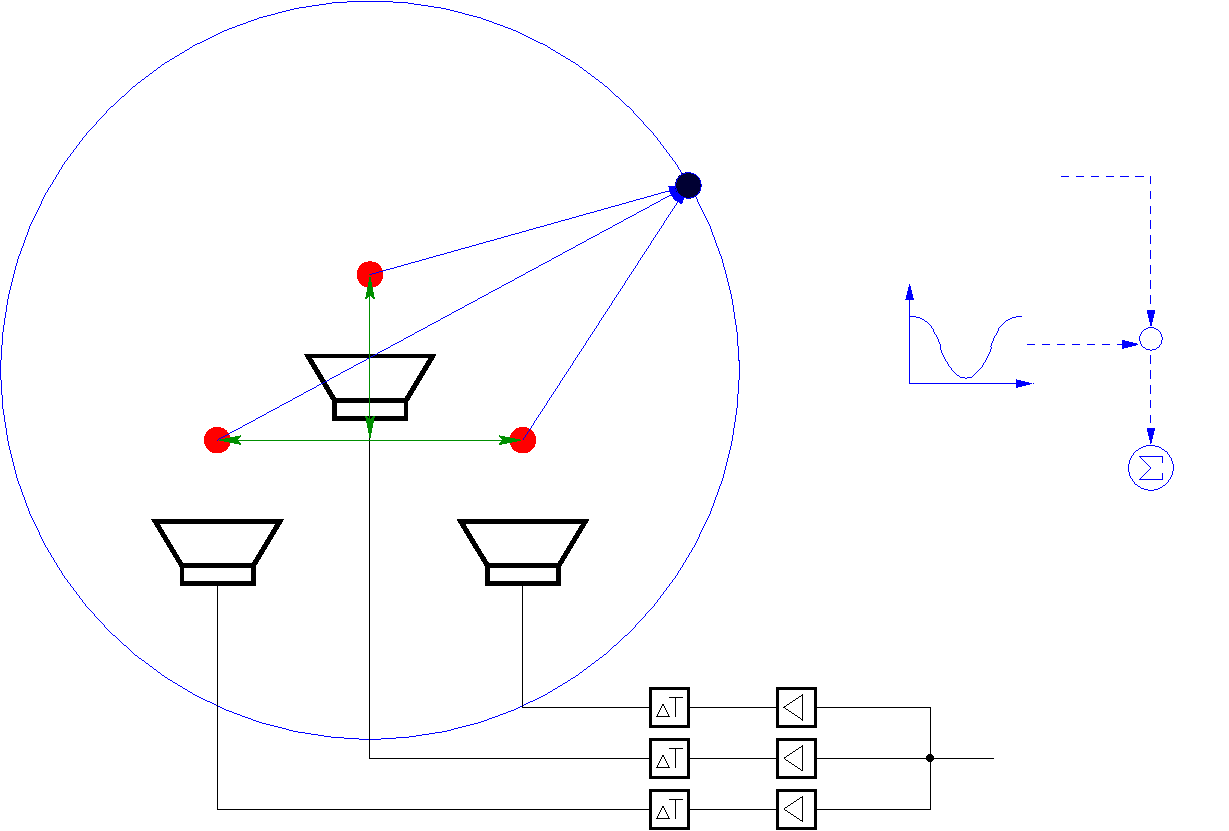
\includegraphics{genetic_setup_01.pdf}%
\end{picture}%
\setlength{\unitlength}{3937sp}%
\begingroup\makeatletter\ifx\SetFigFont\undefined%
\gdef\SetFigFont#1#2#3#4#5{%
  \reset@font\fontsize{#1}{#2pt}%
  \fontfamily{#3}\fontseries{#4}\fontshape{#5}%
  \selectfont}%
\fi\endgroup%
\begin{picture}(9844,6664)(-681,-4729)
\put(8502,-884){{\color[rgb]{0,0,1}*}%
}
\put(2701,-1411){{\color[rgb]{0,0,0}Speaker A}%
}
\put(1441,-2761){{\color[rgb]{0,0,0}Speaker B}%
}
\put(3871,-2761){{\color[rgb]{0,0,0}Speaker C}%
}
\put(5941,-3661){{\color[rgb]{0,.56,0}\texttt{Va}}%
}
\put(5941,-4066){{\color[rgb]{0,.56,0}\texttt{Vb}}%
}
\put(5941,-4471){{\color[rgb]{0,.56,0}\texttt{Vb}}%
}
\put(4906,-4471){{\color[rgb]{0,.56,0}\texttt{Phic}}%
}
\put(4906,-4066){{\color[rgb]{0,.56,0}\texttt{Phib}}%
}
\put(4906,-3661){{\color[rgb]{0,.56,0}\texttt{Phia}}%
}
\put(2341,-601){{\color[rgb]{0,.56,0}\texttt{Ly}}%
}
\put(1081,-331){{\color[rgb]{1,0,0}Ac. Center A}%
}
\put(-179,-1681){{\color[rgb]{1,0,0}Ac. Center B}%
}
\put(3691,-1681){{\color[rgb]{1,0,0}Ac. Center C}%
}
\put(5131,659){{\color[rgb]{0,0,1}Pressure along the circumference}%
}
\put(5131,404){{\color[rgb]{0,0,1}of the array, calculated according}%
}
\put(5131,149){{\color[rgb]{0,0,1}to the augmented pressure equation \ref{eq:aug_omni}}%
}
\put(1801,-1771){{\color[rgb]{0,.56,0}\texttt{Lx}}%
}
\put(6436,-1366){{\color[rgb]{0,0,1}weighting curve}%
}
\put(8056,-2176){{\color[rgb]{0,0,1}fitness value}%
}
\end{picture}%
	\end{minipage}
	\end{sideways}
%\center
\caption{Phenotype and Genotype relations, visualization of genes and fitness evaluation. Genotype parameters are denoted in \textcolor{green3}{green} and the fitness evaluation method is denoted in \textcolor{blue}{blue}.}
\label{fig:gene_setup}
\end{figure}
In order to set up a \gls{ga}, the \textit{phenotypes}, which are real world solutions to the real world problem, have to be coded into \textit{genotypes}, which represent those solutions in a mathematical domain. This corresponds to the coded parameter sets that are mentioned in point 1. in \autoref{sec:ga_fundamental}.
A way to describe the acoustical beamforming problem, that this project is investigating, is illustrated in \autoref{fig:gene_setup}. The parameters, that make up the genotypes, are denoted in \textcolor{green3}{green} letters. The hardware setup consists of three loudspeakers (A,B,C). Each of the speakers is fed a signal, that is a modified version of a common source signal. The signals differ in gain (\textcolor{green3}{\texttt{Va}}, \textcolor{green3}{\texttt{Vb}}, \textcolor{green3}{\texttt{Vc}}) and phase (\textcolor{green3}{\texttt{Phia}}, \textcolor{green3}{\texttt{Phib}}, \textcolor{green3}{\texttt{Phic}}). The positioning of the \textcolor{red}{acoustic centers} of the loudspeakers relative to each other is set up as a isosceles triangle. The triangle is described using the length of its base side (\textcolor{green3}{\texttt{Lx}}) and the corresponding height (\textcolor{green3}{\texttt{Ly}}). Negative values of \textcolor{green3}{\texttt{Ly}} mean, that the tip of the triangle is pointing in the opposite direction compared to the setup in \autoref{fig:gene_setup}. When speaking about genetic algorithm, the formerly mentioned parameter are commonly refered to as \textit{genes}. The particular value, that each of the genes has in a genotype is referred to as an \textit{allele}. The set of genes are refered to as \textit{chromosomes}. In this particular case, each individual genotype has just one chromosome and the alleles are represented in float values.\\
Because the genetic algorithm works on with a pool of solutions at any given time, it is necessary to initialize a population of genotypes. This corresponds to point 2. in \autoref{sec:ga_fundamental}. The way, that the population is initialized in the algorithm used for this project, is shown in Appendix \ref{axs:pop_init}. The initial alleles are determined with some random values that are combined with some educated guessing (see also \autoref{sec:ga_prior}).\\
According to point  3. in \autoref{sec:ga_fundamental} there needs to be a function that evaluates the fitness of every genotype based on some criteria. The way that this is achieved is also visualized in \autoref{fig:gene_setup}. The corresponding code is shown in Appendix \ref{axs:fitness}. The coordinates of a \textcolor{blue}{circle} around the centroid of the triangle between the \textcolor{red}{acoustic centers} are calculated. The radius of the circle is signficantly bigger then the size of the speaker array. From these circle coordinates a set of coordinates, that describes the distance to each \textcolor{red}{acoustic center}, is deducted for every one of the speakers. Using these coordinates and the gain and phase parameters from the alleles as well as the frequency, for which the optimization is excecuted, the pressure from each speaker is calculated using \autoref{eq:aug_omni}. The (complex) pressures are added in order to get the resulting pressure along the circumference.\\
The ultimate goal of running this \gls{ga} is getting phenotype solution, that leads to a particular desired directional characteristic of the speaker array. This is implemented, by weighting the normed pressure along the circumference according to some preferences. This means, pressure in the direction in the direction, in which sound emission is desired, is assigned a low cost, whereas pressure in a direction, in which sound emission is undesired, is assigned a high cost. When the normed and weighted pressure is summed, a fitness value is put out. The formerly described way of applying weight leads to lower values corresponding to fitter solutions.\\
The final point 4. from \autoref{sec:ga_fundamental} mentions probabilistic transition rules. The implementation of these is shown in Appendices \ref{axs:parents}, \ref{axs:offspring} and \ref{axs:mutation}. The genotypes, that are used to generate new genotypes for the subsequent generation are selected via tournament
selection \citep{tournament}. This ensures plenty of randomness while there is still some pressure caused by the fitness of the individual solution.
Offspring is then generated by combining the alleles of the parent genotype at a randomly determined ratio. This leads to two offspring genotypes with complementary ratios.
Furthermore there is a mutation function, that, with a comparatively low probability, changes one of the alleles of any genotype to a randomly determined value.\\
A number of generations are computed after the initialization. The most fit genotype of the last generation that is computed should represent a near optimal solution to the beamforming problem. It has to be noted, that this routine has to be repeated for every frequency, for which a set of parameters is to be obtained.



\section{Inclusion of Prior Knowledge}\label{sec:ga_prior}
To simplify the optimization task, it is expedient to exploit knowledge and requirements given from the context of the project. This prior knowledge contains constraints that are given by practical issues. This leads to constraints, like the maximum distance between the acoustic centers, that is determined by the size of the anechoic chamber, in which the speaker array should be set up for measurements, or the minimum distance between the acoustic centers, which is determined by the physical size of the loudspeakers. It is possible to use the optimization to obtain parameters that lead to a main emission direction of the speaker array in any direction. However, for practical reasons the preferred solution has either a single speaker on the line between the centroid of the triangle that makes up the array and main emission direction, or the connecting line between to acoustic centers perpendicularly to the formerly mentioned main emission direction. This leads to a symmetrical array configuration, which means, that optimal signal processing parameters are highly likely to be equal for two of the three speakers. Implementing this, the optimization can be simplified.
Another form of prior knowledge is used when initializing the population. With trial-and-error style heuristics, some knowledge about the nature of fit solutions can be gained and implemented in the initialization function as an expectational value when setting up parameters as Gaussian random variables.\\
Prior knowledge is also incorporated in the way that the optimization is excecuted over the whole frequency range of \SIrange{60}{300}{\hertz}. Heuristic trials have shown, that the placement of the loudspeakers is much more critical for the optimization result at higher frequencies then it is at lower frequencies. When it is intended to actually set up a speaker array that is driven the signal processing parameters that are the result of the optimization process, and measure and experience the performance, then it is not feasible to have different speaker positions for different frequencies. For this reason the optimization process is startet at the highest frequency. The speaker position is then fixed. In the following optimization runs, only gain and phase are optimized. Using the population of the last generation from the previous frequency optimization, allows to have a smaller number of generations when optimizing for the adjacent frequency as many of the genotypes are already close to optimal.

\section{Optimization Results}\label{sec:opt_result}
The best genotypes for every frequency can be used, to generate polar plots of the expected directional characteristics. Generating these is done similarly to the fitness evaluation by calculating the normed summed pressure along a circumference using \autoref{eq:aug_omni}.
For a setup with the corner of the array pointing towards the main emission direction, the expected directional characteristics are shown in \autoref{fig:expected_pcor}.\\
\begin{figure}[H]
	\centering
	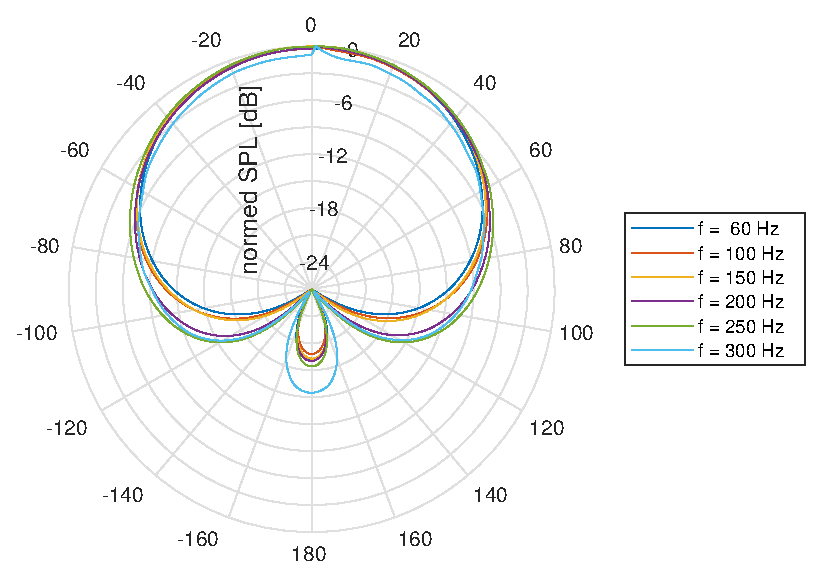
\includegraphics[width=0.7\textwidth]{expected_polar_pcor.eps}
	\caption{Expected directional characteristics, optimization with pressure corrected cost function, correction table based on Appendix \ref{ax:directional_2}, generation count: $N_{start}=60$, $N_{rest}=30$, population size $t=1250$, \textcolor{green3}{\texttt{Lx}}\,$=$\,\SI{0.405}{\meter}, \textcolor{green3}{\texttt{Ly}}\,$=\,$\SI{0.249}{\meter}}
		\label{fig:expected_pcor}
\end{figure}
\begin{figure}[H]
	\centering
	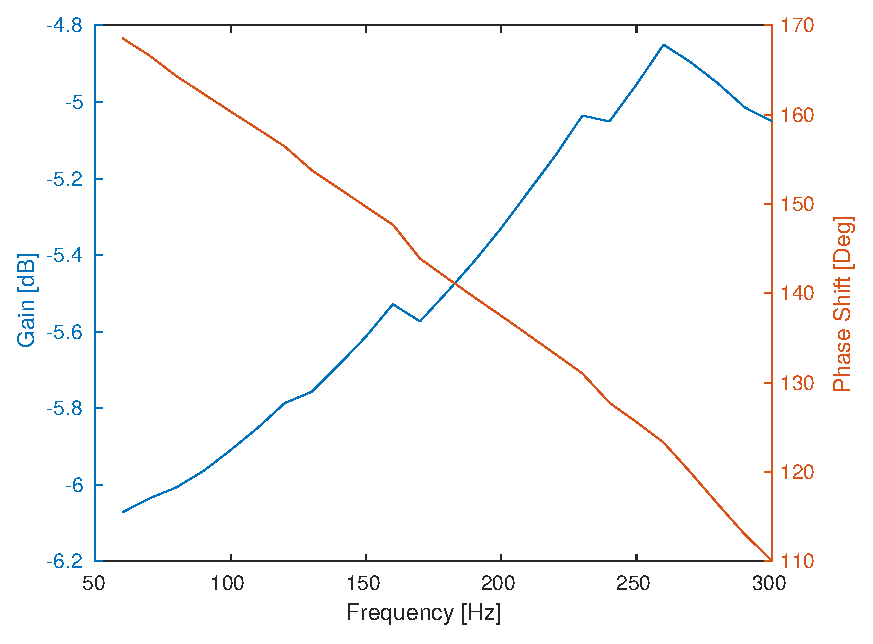
\includegraphics[width=0.7\textwidth]{filter_req.eps}
	\caption{Amplitude and phase for loudspeakers B and C, relative to loudspeaker A, corresponding to the expected behaviour shown in \autoref{fig:expected_pcor}}
		\label{fig:filter_req}
\end{figure}

\section{Main axis response}
The aim of this section is to compare the response of the optimized cardioid speaker model with a line of speakers which radiate the same sound with the same parameter. The transfer function in the front of the cardioid speaker array might not have the same transfer function compare to the line of speakers. Therefore the pressure in the front might be a cost when going from speaker array that radiate omnidirectional to make them radiate with a cardioid patten. The cost can be frequency dependent and therefore the transfer function in the front is changed. It is interesting to investigated the pressure in the front of a line of three speaker, where they all have the same parameters compare to the cardioid speaker model, since the cardioid speaker model is made of three speaker unit. The cost of the cardioid model compared to the three speaker on a line will be analysed analytical in this section and end out with the needed parameter for making a flat frequency response in the front of the speaker array and a conclusion of the power loose. To make this comparing, a transfer function is made of both model from \SI{60}{\hertz} to \SI{300}{\hertz}. The difference between thoes two model is then defined as the cost. To do so, an analytical speaker model of one speaker have to be developed such that it have a flat frequency response in the frequency of interest. The speaker model will be a pulsating sphere with a radius of \SI{33}{\centi\meter} where the non linear frequency response is compensated such that the speaker model have a flat frequency response from  ke this comparing, a transfer function is made of both model from \SI{60}{\hertz} to \SI{300}{\hertz}. The pressure in the front of the three alined model might also be frequency dependent, but the frequency where the pressure is lowest will then be used as the reference pressure \\

The main axis response of the three alined speaker is analysed analytical at a distance of \SI{10}{\meter} from the array center. The array center is the median cross of the cardioid speaker array model, which than mean that the speaker position in the alined model is as in the cardioid speaker model, but only where the back speaker is moved to the front line. All three speaker is radiation with a pressure of \SI{1}{\pascal} and the pressure at the main axis at a distance of \SI{10}{\meter} from the array center is the reference pressure point. \autoref{fig:ref_omni_array} shows the alined model, where it can be seen that the array center is behind the acoustical speaker alinement. All speaker have a time delay of zero and a frequency depended velocity 

\begin{figure}[h]
	\centering
\begin{picture}(0,0)%
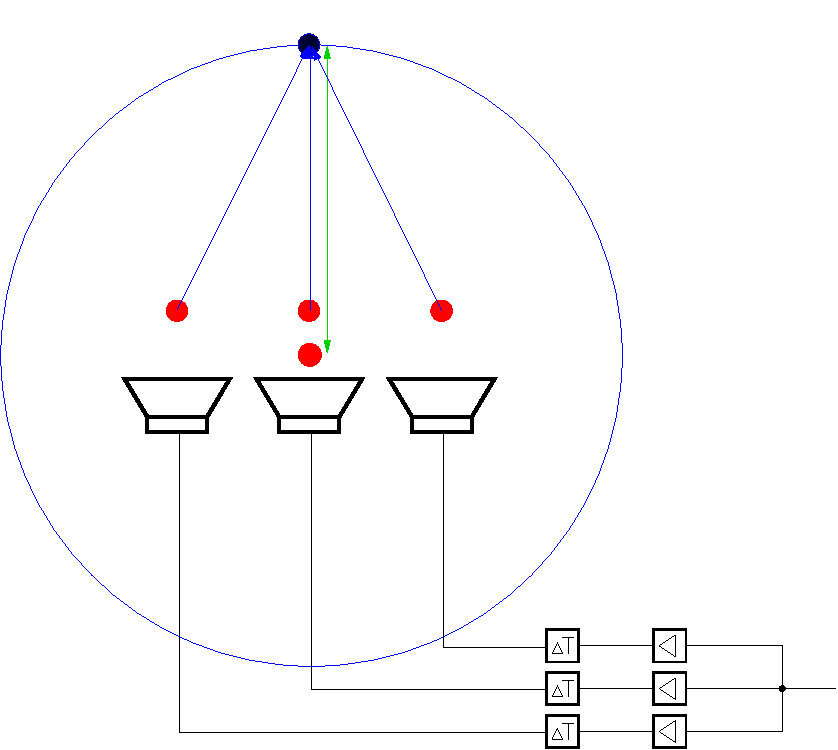
\includegraphics{ref_omni_array.pdf}%
\end{picture}%
\setlength{\unitlength}{3315sp}%
%
\begingroup\makeatletter\ifx\SetFigFont\undefined%
\gdef\SetFigFont#1#2#3#4#5{%
  \reset@font\fontsize{#1}{#2pt}%
  \fontfamily{#3}\fontseries{#4}\fontshape{#5}%
  \selectfont}%
\fi\endgroup%
\begin{picture}(7975,7142)(-672,-4729)
\put(1711,-331){\color[rgb]{1,0,0}Ac. Center A}%
\put(5941,-3661){\color[rgb]{0,.56,0}\texttt{V}}%
\put(5941,-4066){\color[rgb]{0,.56,0}\texttt{V}}%
\put(5941,-4471){\color[rgb]{0,.56,0}\texttt{V}}%
\put(4906,-4471){\color[rgb]{0,.56,0}\texttt{0}}%
\put(4906,-4066){\color[rgb]{0,.56,0}\texttt{0}}%
\put(4906,-3661){\color[rgb]{0,.56,0}\texttt{0}}%
\put(2271,2230){\color[rgb]{0,0,0}$L_{p,ref}$}%
\put(2535,219){\color[rgb]{0,.82,0}\SI{10}{\meter}}%
\put(-409,-601){\color[rgb]{1,0,0}Ac. Center B}%
\put(3736,-601){\color[rgb]{1,0,0}Ac. Center C}%
\put(1081,-1906){\color[rgb]{0,0,0}Speaker B}%
\put(2341,-1906){\color[rgb]{0,0,0}Speaker A}%
\put(3601,-1906){\color[rgb]{0,0,0}Speaker C}%
\put(2476,-1051){\color[rgb]{1,0,0}Array center}%
\end{picture}%
	\caption{Configuration for reference pressure $L_{p,ref}$.}
		\label{fig:ref_omni_array}
\end{figure}

The following graph \autoref{fig:graph_plot_three_line} shows the absolute pressure from \SI{60}{\hertz} to \SI{300}{\hertz} of the aligned speaker model. 

\begin{figure}[H]
	\centering
	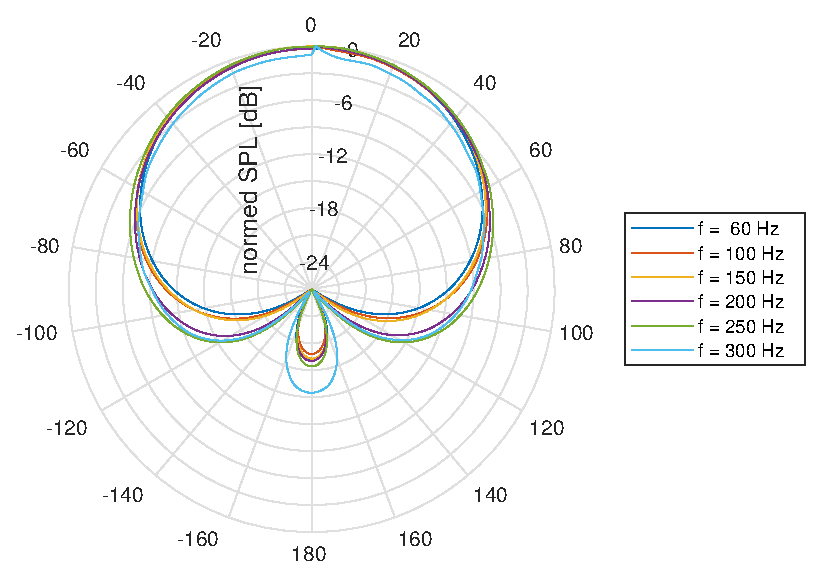
\includegraphics[width=0.7\textwidth]{expected_polar_pcor.eps}
	\caption{The graph shows the frequency response of the aligned speaker model from \SI{60}{\hertz} to \SI{300}{\hertz}}
		\label{fig:graph_plot_three_line}
\end{figure}

From the graph in \autoref{fig:graph_plot_three_line} it can be seen that the pressure reference point is frequency dependent, when alining three speaker in an array with the same parameters, but the frequency dependency is small. The used 






\begin{figure}[h]
	\centering
\begin{picture}(0,0)%
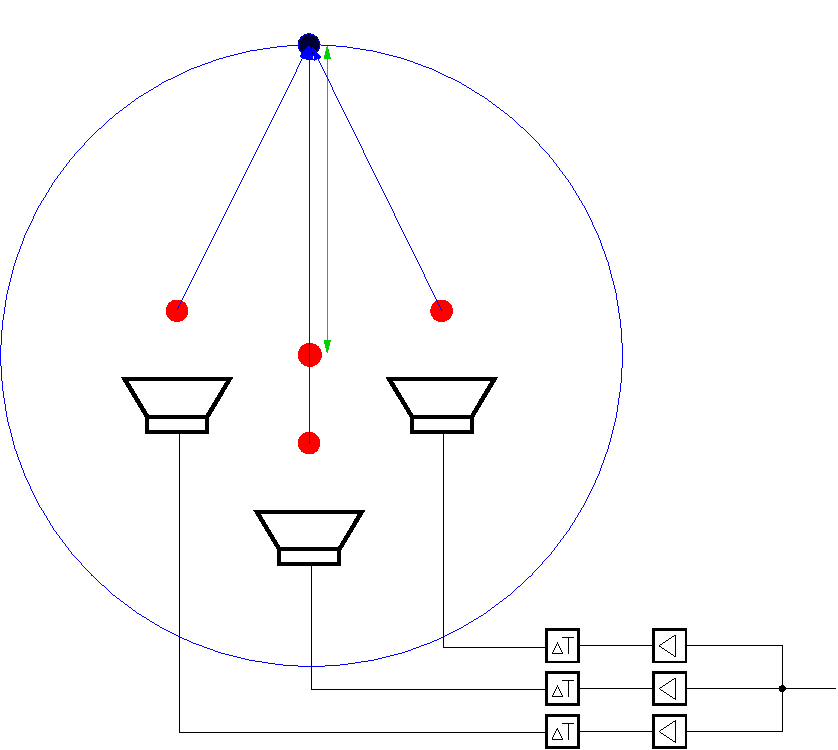
\includegraphics{ref_caridioid_array.pdf}%
\end{picture}%
\setlength{\unitlength}{3315sp}%
%
\begingroup\makeatletter\ifx\SetFigFont\undefined%
\gdef\SetFigFont#1#2#3#4#5{%
  \reset@font\fontsize{#1}{#2pt}%
  \fontfamily{#3}\fontseries{#4}\fontshape{#5}%
  \selectfont}%
\fi\endgroup%
\begin{picture}(7975,7142)(-672,-4729)
\put(5941,-3661){\color[rgb]{0,.56,0}\texttt{Va}}%
\put(5941,-4066){\color[rgb]{0,.56,0}\texttt{Vb}}%
\put(5941,-4471){\color[rgb]{0,.56,0}\texttt{Vb}}%
\put(4906,-4471){\color[rgb]{0,.56,0}\texttt{Phic}}%
\put(4906,-4066){\color[rgb]{0,.56,0}\texttt{Phib}}%
\put(4906,-3661){\color[rgb]{0,.56,0}\texttt{Phia}}%
\put(2271,2230){\color[rgb]{0,0,0}$L_{p,ref}$}%
\put(2535,219){\color[rgb]{0,.82,0}\SI{10}{\meter}}%
\put(2566,-1051){\color[rgb]{1,0,0}Array center}%
\put(2386,-3211){\color[rgb]{0,0,0}Speaker A}%
\put(1756,-2086){\color[rgb]{1,0,0}Ac. Center A}%
\put(-179,-601){\color[rgb]{1,0,0}Ac. Center B}%
\put(-181,-1906){\color[rgb]{0,0,0}Speaker B}%
\put(3736,-601){\color[rgb]{1,0,0}Ac. Center C}%
\put(3646,-1906){\color[rgb]{0,0,0}Speaker C}%
\end{picture}%
	\caption{.}
		\label{fig:ref_caridioid_array}
\end{figure}






